\chapter{Results}
\label{chapter:results}
In this chapter, we apply the advanced statistical tools to the heavy-flavor transport model and extract the heavy quark transport coefficients.
I would like to present this in a two step processes to show the improvements of the lastest extraction.



\paragraph{A list of experimental data}
\begin{center}
\begin{table}[h]
\caption{ALICE dataset}\label{table:ALICE-obs} 
\begin{tabularx}{\columnwidth}{XXX}
\hline 
 Observables & Centrality & Reference\\ 
\hline 
$D$-meson $v_2$ & 30-50\% & {Acharya:2017qps}\\ 
\hline 
Event-engineered $D$-meson $v_2$ & 30-50\% & {Grosa:2017zcz}\\ 
\hline 
$D$-meson $R_{AA}$ & 0-10, 30-50, 50-80\% & {Acharya:2018hre}\\
\hline 
\end{tabularx}
\end{table}
\begin{table}[h]
\caption{CMS dataset}\label{table:CMS-obs} 
\begin{tabularx}{\columnwidth}{XXX}
\hline 
Observables & Centrality & Reference\\ 
\hline 
D${}^0$-meson $v_2$ & 0-10, 10-30, 30-50\% & {Sirunyan:2017plt}\\ 
\hline 
D${}^0$-meson $R_{AA}$ & 0-10\%, 0-100\% & {Sirunyan:2017xss}\\ 
\hline 
B${}^{\pm}$-meson $R_{AA}$ & 0-100\% & {Sirunyan:2017oug}\\ 
\hline 
\end{tabularx}
\end{table}
\end{center}

\section{Lessons from earlier extractions of $\hat{q}_Q$}
In an earlier publication [], we used a linearized Boltzmann model with the coherence factor approach to implement the LPM effect.
The heavy quark initial momentum dsitribution is obtained from the FONLL calculation.
We have already commented on the advantages and disadvantages of these choices.
Two different set of nuclear PDF $EPPS$ and $nCTEQ15$ are used to represent the uncertainty from the cold nuclear matter effect in the $\hat{q}$ extraction.

Regarding model parameters, the one parameter for the perturbative elastic and inelastic scatterings is controlled by $1/3 < \mu < 4$ in the running coupling. 
There is an additional pure diffusion process with a diffusion constant $\kappa_{NP}$ parametized to peak at low temperature and low energy, in order to mimic certain non-perturbative coupling between a low energy probe and the medium near $T_c$,
\begin{eqnarray}
\kappa_{NP} = T^3 \kappa_D \left(x_D + (1-x_D)\frac{1\textrm{ GeV}{}^2}{ET}\right).
\end{eqnarray}
The $0<\kappa_D<8$ parameter is the overall strength of the diffusion, and the $0<x_D<1$ controls the degree of energy-temperature dependence.
One can see that in the heavy quark limit $M\rightarrow \infty$, this parametrization becomes independent of mass.
An additional parameter is the in-medium energy loss starting time $\tau_0$ that is allowed to be tuned between $0.1$ fm/$c$ to $1.0$ fm/$c$ (before the onset of hydrodynamics).
The reason is we lack a quantitative description of the production of color charge in the initial stages.
This starting time is a simple approximation that interactions is only turned on after $\tau_0$ when the color carries is assumed to approach a Boltzmann distribution.


The design of the four dimensional parameter space  $(\tau_0, \mu, \kappa_D, x_D)$ has 80 design points.
The computation is carried on the distributed computing system Open Science Grid [] using about a million CPU hours.
The observabes on which we calibrated are listed in tables \ref{table:ALICE-obs} and \ref{table:CMS-obs}. 
Including, $p_T$ dependent $D$-meson nuclear modification factor $R_{AA}$ and $p_T$ dependent (event-shape-engineered) azimuthal anisotropy $v_2$.
CMS measurements of the $B^{\pm}$-meson $R_{AA}$ is also included to constrain the mass dependence of the transport coefficients.

\begin{figure*}
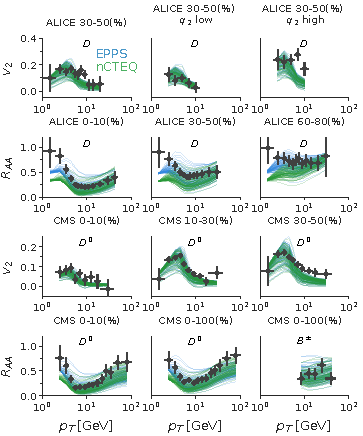
\includegraphics[width=.49\textwidth]{observables_design.pdf}
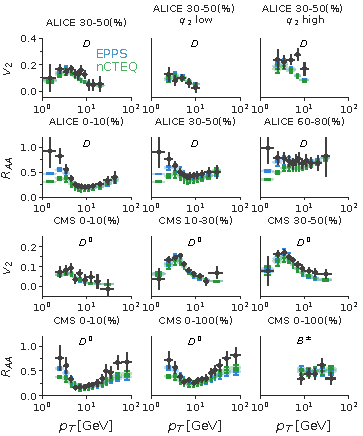
\includegraphics[width=.49\textwidth]{observables_posterior.pdf}
\caption{Left: the prior, i.e. the full range of calculations in parameter space. Right: the posterior, i.e. observables sampled from model emulators after calibration. In both figures, blue (green) lines are calculations with {\tt EPPS} ({\tt nCTEQ15np}) nuclear PDF.}\label{plots:deisgn_posterior_obs}
\end{figure*}

The prior and the posterior of the observables before and after the calibration is shwon in figure \ref{plots:deisgn_posterior_obs}.
blue stands for using {\tt EPPS} nuclear PDF and green stands for using the {\tt nCTEQnp}  nuclear PDF.
We found that the model after the calibration provide a good description of $R_{AA}$ and $v_2$ at the intermediate $p_T$ of the ALICE experiments.
But it does not reproduce the fast uprising shape of $R_{AA}$ at high-$p_T$ of the CMS experiment.
In addition, the model seem to under estimate the high-$p_T$ $v_2$ of the $30-50\%$ centrality bin measured by CMS.
The model is able to explain the correlation between the D-meson $v_2$ and the event-shape, though there are still large fluctuation in the data.
The use of different nuclear PDFs has a negligible effect on $v_2$, but does affect the $R_{AA}$ at small and large $p_T$.
Another thing worth noting that is that the $D$ and $B$ meson $R_{AA}$ are described at the same time.

\begin{figure}
\centering
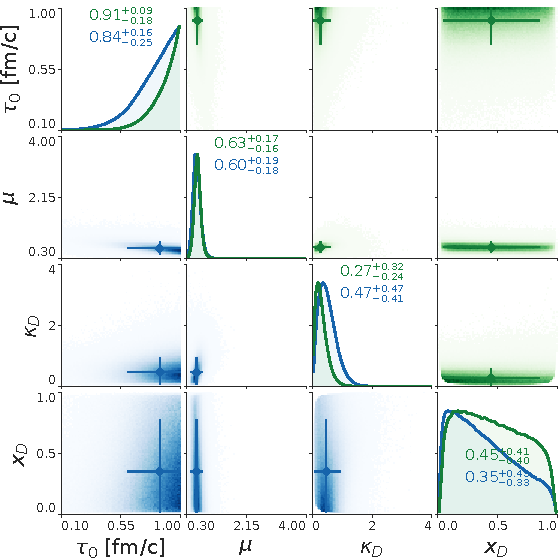
\includegraphics[width=.7\textwidth]{posterior.pdf}
\caption{Marginalized postrior probability distribution of model parameters. Diagonal plots show the marginalization on a single parameter. Off diagonal plots show the pair correlation between parameters. Blue (Geen) lines and lower (upper) off diagonal plots correspond to the extraction using EPPS (nCTEQ15np) nuclear PDF.}\label{plots:posterior}
\end{figure}

The inferred posterior probability distribution of the parameters is shown in the figure \ref{plots:posterior}.
The diagonal plots show single parameterized distributions, and the off-diagonal ones displays the two-parameter correlations.
We split the results that use different nuclear PDFs into the upper (EPPS, green heat map and lines) and lower (nCTEQ15np, blue heat maps and lines) triangles.
One notices that results from different nuclear PDF are consistent within the uncertainty; therefore, from now on I shall not stress on any differences between these two set of results, but combine them into a single distribution to fold in the PDF uncertainty.
The favored parameters are $\mu \sim 0.6$ and $\kappa_D \sim 0.4$, indicating a large in-medium $\alpha_s$ and a small additional diffusion.
The typical value of the $\alpha_s$ is, in fact, so large that let one worried about the use of weakly-couple based approaches.
For example, $\alpha_s(0.6\pi T)$ at $T=300$ MeV is 0.67, corresponding to $g \approx 3$. 
And the screening mass $m_D \sim 3.6 T$ is even larger than the average energy of the thermal partons $3T$. 
In the discussion of the next section, we will see that this problem can be slightly alleviated, once we use the improved implementation of the LPM effect and implement a separation of soft-modes into the diffusion constant, though $g$ is still large.

\begin{figure}
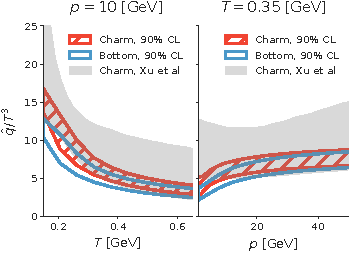
\includegraphics[width=\columnwidth]{qhat_p_T.pdf}
\caption{Posterior range of the heavy quark transverse momentum broadening parameter $\hat{q}$ from Equation \ref{eq:qhat}. The results include the uncertainty from using different nuclear PDFs. Blue boxed region is for bottom quarks and red slashed region for charm quarks.}\label{fig:posterior_qhat}
\end{figure}

\paragraph{Transport coefficients} In this analysis, the heavy quark transport coefficient $\hat{q}$ is computed from adding up the momentum broadening from both the scattering and the parametric diffusion,
\begin{eqnarray}\label{eq:qhat}
\hat{q} &=& 2T^3\kappa_D\left(x_D + (1-x_D)\frac{\textrm{GeV}^2}{ET}\right) + \hat{q}_{\textrm{el}}.
\end{eqnarray}
In a perturbative definition of the transport coefficients, the inelastic process does not contribute to heavy quark transport coefficient at leading order. 
In figure \ref{plots:posterior_qhat}, the 90\% credible region of $\hat{q}$ is shown as a function of temperature at a fixed energy (left), and as function of energy at a fixed temperature (right).
Results for charm (red) and bottom (blue) quarks are labeled by different colors.
The mass difference only causes a small difference in $\hat{q}$.

\begin{figure}
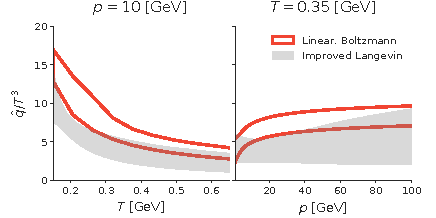
\includegraphics[width=\columnwidth]{qhat_compare.pdf}
\caption{Posterior range of the heavy quark transverse momentum broadening parameter $\hat{q}$. The shaded region indicates a previous extraction using the improved-Langevin model [].}\label{fig:compare_qhat}
\end{figure}

\paragraph{Comparison to results from an improved-Langevin model}
The same transport coefficient is also extracted using the improved-Langevin model [].
It includes a diffusion modeling of the elastic interacton, a high-twist single gluon emission rate, and a similar routine to implement multiple radiations.
This model is then coupled to the same medium as the one used here and compared to the same set of observables as this work does.
The resultant posterior (for charm quark only) is shown as the shaded region in figure \ref{fig:compare_qhat}.
We see that the $\hat{q}$ extracted using the two models only overlap at the boundary of the credible region.
Their difference is comparable to the uncertainty band of either model, while both models provide a reasonable description of the data.
This suggests the theoretical uncertainty that comes from the assumption between the probe and the medium is a significant one.
The ability to tune a switching scale parameter in the new model intends to include this type of theoretical uncertainty.

\section{Calibration with the improved transport model}
Finally, we apply the improved model to the extraction of the heavy quark transport coefficients.
As a summary of the improvements:
\begin{itemize}
\item A more sophisticated implementation of the LPM effect to reduce modeling uncertainty of the radiative process;
\item An interpolation of the diffusion picture and the scattering picture to take into account modeling uncertainty.
\item Restrict the use of few-body matrix-elements to only large-$Q$ interactions.
\item Separating the high-virtuality evolution and the low-virtuality transport equation at a medium scale.
\end{itemize}


\paragraph{Model parameters}
In the new analysis, we try to include as many theoretical uncertainty as possible, therefore we have much more parameters than the two previous efforts.
They are listed in table \ref{table:new:prior}.
The first parameter is still the energy loss starting time $\tau_i$, it is the moment one believe the medium is opaque enough to employ the linearized transport model.
The second parameter is switching scale parameter $c$ as in $Q_{\textrm{cut}}^2 = c m_D^2$, it is allowed to be vary between $0.1 and 10$.
The third parameter control at medium-scale at which the vacuum-like radiation matches to a medium-induce radiation calculation, in chapter \ref{coupling}, we have been using the criterion $k_\perp = \Delta k_\perp^2$ as the matching point.
But since this is only a qualitative argument, we should allow this condition to vary around this na\"ive expectation $k_\perp = R_v \Delta k_\perp^2$.
$R_v$ can vary between 0 and 7.
Again, a $\mu$ parameter controls the in-medium strong coupling $\alpha_s = \alpha_s(\max\{Q, \mu\pi T\})$.
The rest of the six parameters $K,a,b,p,q, \gamma$ parametrizes a correction to the weakly coupled motivated transport coefficient modeled by diffusion. 
Its origin can be either perturbative or non-perturbative and this additional transport coefficient is,
\begin{eqnarray}
\frac{\Delta\hat{q}}{T^3} &=& \frac{K}{\left[1+\left(a\frac{T}{T_c}\right)^p\right]\left[1+\left(b\frac{E}{T}\right)^q\right]}
\end{eqnarray}
$K$ is the overall magnitude of the correction. $a$ and $p$ parametrize an deviation from the $T^3$ scaling of the $\hat{q}$ near $T_c$, while $b$ and $q$ parametrize the energy dependence.
We also allow this additional transport parameter to be anisotropic ($\Delta\hat{q}\neq 2\Delta\hat{q}_L$)
\begin{eqnarray}
\Delta\hat{q}_L &=& \frac{\Delta\hat{q}}{2} \left(\frac{E}{M}\right)^{\gamma}.
\end{eqnarray}
And the $\gamma$ parameter is allowed to vary from $-1$ to $1$.
Note that such a construction goes back to an isotropic diffusion when velocity approaches zero ($E\rightarrow M$).

\begin{table}
\centering
\caption{Prior range of parameters}\label{table:new:prior}
\begin{tabular}{ccc}
\hline
Symbol & Description & Range \\
\hline
$\xi = \frac{\tau_0}{\tau_{\textrm{hydro}}}$ & Energy loss starting time & (.1, .9) \\
$c = \frac{Q_{\textrm{cut}}^2}{m_D^2}$ & Soft / hard switching scale & $(.1, 10.)$ \\
$R_v = \frac{k_\perp^2}{\Delta k_\perp^2}$ & Vacuum / Medium mathcing scale & $(0.14, \infty)$\\
$\mu$ & Running $\alpha_s$ stops at $Q = \mu\pi T$ & $(.6, 10)$ \\
$K$ & Magnitude of $\Delta \hat{q}/T^3$ & $(0, 20)$\\ 
$p$ & \multirow{2}{*}{$E$-dependence of $\Delta \hat{q}/T^3$} & $(-2, 2)$\\ 
$a$ &  & $(-1, 1)$\\ 
$q$ & \multirow{2}{*}{$T$-dependence of $\Delta \hat{q}/T^3$}  & $(-.5, 3)$\\ 
$b$ &   & $(-.5, 3)$\\ 
$\gamma$ & $\Delta \hat{q}_L = (E/M)^\gamma\Delta \hat{q}_L$  & (-1, 1)\\ 
\hline
\end{tabular}
\end{table}

\paragraph{Design and prior} We sampled 250 design points and 50 validation points. 
As a remark, we chosoe to give $c, R_v, \mu, a$ and $b$ an uniform prior in their $\log$ space.
This means that if we transform them back to the original space, the prior distribution will not be flat.
The reason we did these is because these parameters either causes a logarithmic slow change in the model or its prior uncertainty is large that it can be vary by orders of magnitude.
For example, the $\mu$ parameter enters the logarithmic running of $\alpha_s$ and we can rewrite the maximum possible $\alpha_s$ as,
\begin{eqnarray}
\alpha_{s,\max}(T) = \frac{2\pi}{9}\frac{1}{\ln(\mu) + \ln(\pi T/\Lambda_{\textrm{QCD}})}
\end{eqnarray}
Therefore, we choose assign a uniform prior to $\ln(\mu)$ so that $\alpha_s$ also varies notable within the prior range.
As for the $c$ parameter, it controls the boundary of the scattering and diffusion approximation, within a reasonable range of $c$, the diffusion dynamics and the scattering dynamics results in a similar amount of energy loss as has been shown in section [], and difference is seen in more subtle observables, therefore it is also assumed to be flat in the $\log$ space.
For $R_v, a$ and $b$, we did this to allow an order of magnitude change in the parameters as we want to test both the large and small number limits.

\begin{figure}
\centering
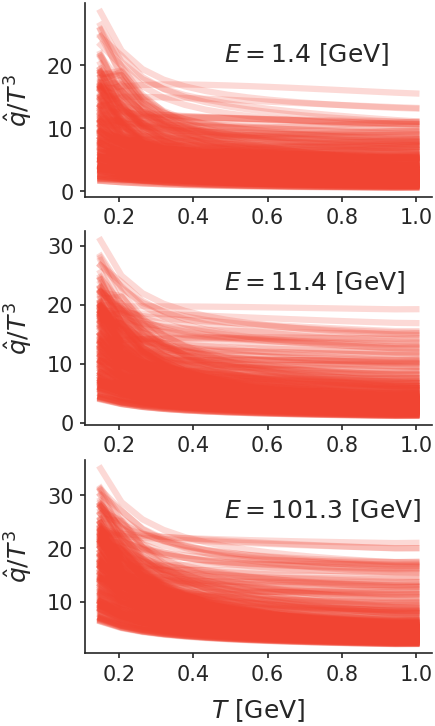
\includegraphics[width=.4\textwidth]{New-analysis/qhat_prior.png}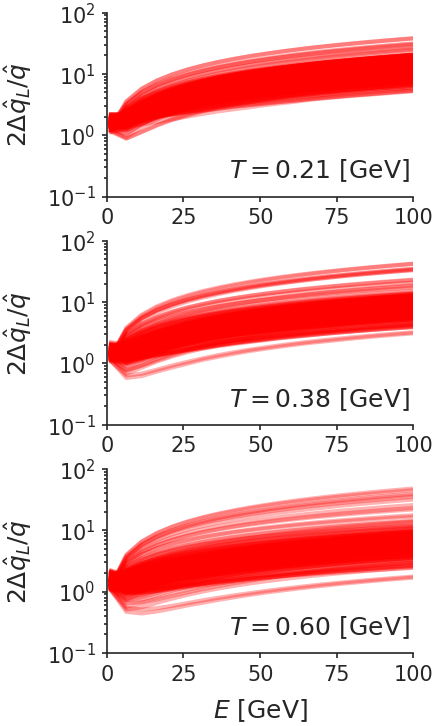
\includegraphics[width=.4\textwidth]{New-analysis/ER_prior.png}
\caption{•}
\label{fig:new:design-qhat}
\end{figure}

To get an idea of what the prior range of the transport parameters looks like, we combine those parameters that enters the computation of the total $\hat{q}$ (including scattering, perturbative diffusion and parametrized correction contribution) and plot them as function of temperature and energy in figure \ref{fig:new:design-qhat}. 
On the left, 250 design's $\hat{q}$ as function of temperatures are shown. Each subplots corresponds to a charm quark energy of $1.4$ GeV, $11.4$ GeV and $101.3$ GeV.
The prior range of $\hat{q}$ varies over a order of magnitude.
On the right of the figure, we show the ratio between the two times of the total $\hat{q}_L$ and $\hat{q}$, if the transport parameters are isotropic, this ratio should be unity.
Due to the inclusion of the large-$Q$ scattering contribution and the parametric correction term, this ratio is not unity so that the prior allows a spectrum of anisotropic transport parameters.
Of course, this ratio always goes to unity when the heavy quark is at rest by construction.

\begin{figure}
\centering
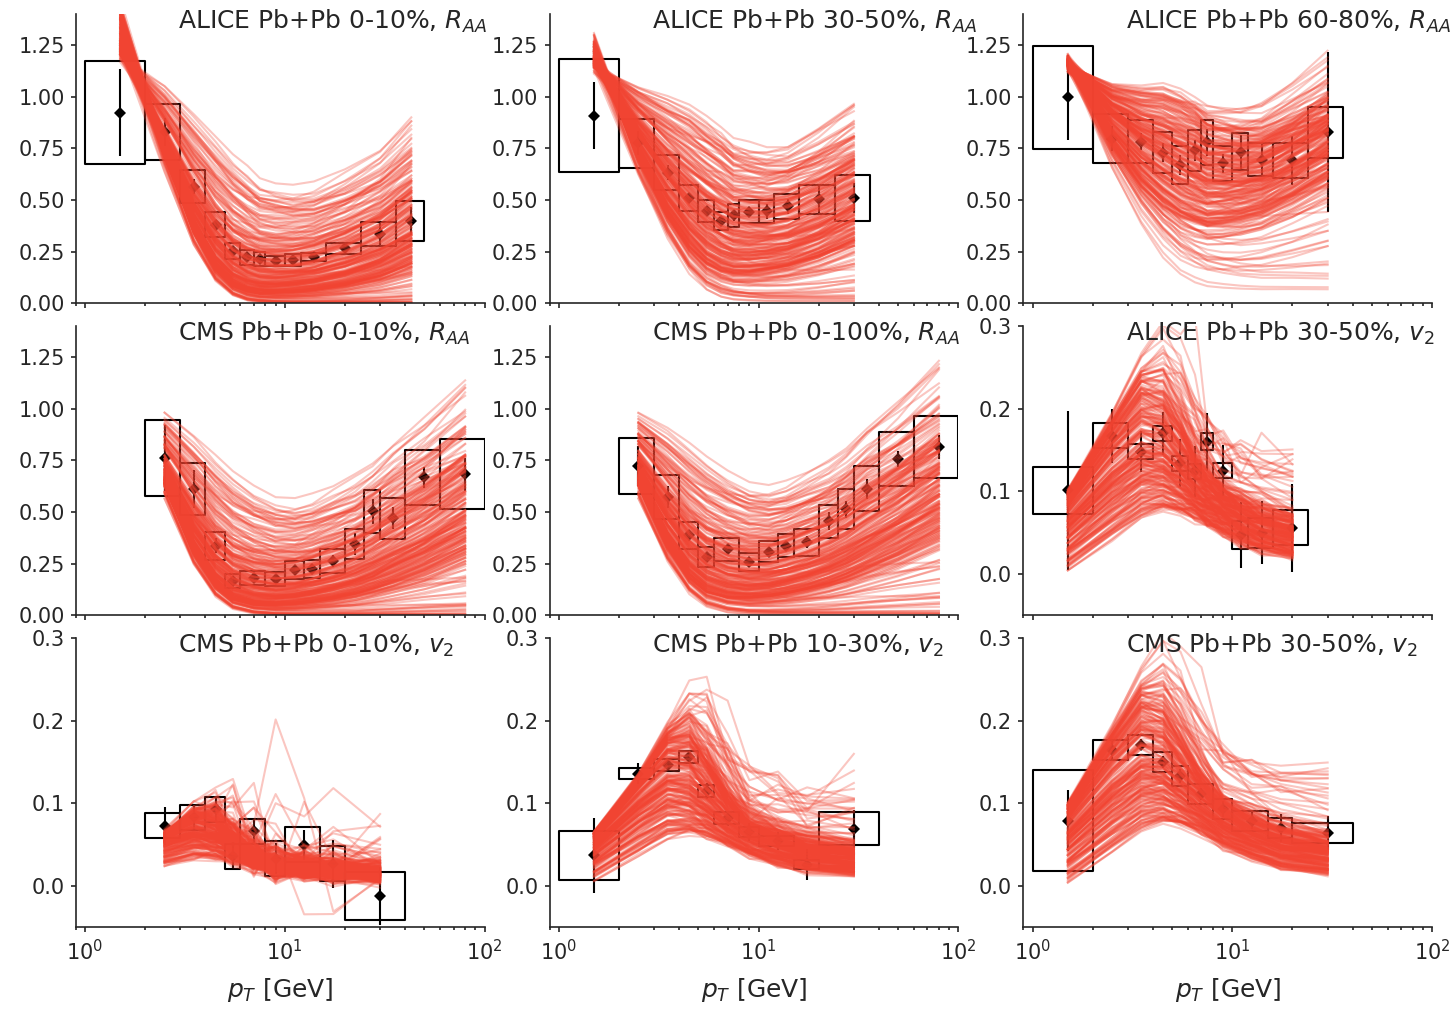
\includegraphics[width=\textwidth]{New-analysis/obs_prior.png}
\caption{•}
\label{fig:new:obs_prior}
\end{figure}

\paragraph{Emulator validation} Computations of the model on both the design points and the validation points are performed on the NERSC super-computing system using over two million CPU hours.
The prior range of the observables are shown in figure \ref{fig:new:obs_prior}.
The $R_{AA}$ and $v_2$ of the heavy flavors are shown, with a good coverage of the data points.
Eight principal components are included, explaining 97.8\% of the data variance.
The validation is then performed on the 50 validation points.
We visualize the validation in figure \ref{fig:new:validation}.
In the top row, the emulated $v_2$ (left) and emulated $R_{AA}$ (right) are compared with the model calculations, and the data from different experiments and centrality has been labeled by different colors.
The emulated values strongly correlates with the true calculations around the the $y=x$ line.
Most points hit off the line, meaning the emulator has uncertainty.
To see if the emulator can reasonably estimate its uncertainty, in the bottom plots, we scatter plot the emulator's standard deviation ($\sigma$) of the prediction (the $y$ axis) versus the absolute value of the true deviation from between the prediction and the calculation (the $x$ axis).
The dashed line defines the shaded region where the true deviation is large than $\pm 3\sigma$.
We found that over $99\%$ of the $v_2$ and $R_{AA}$ points are within the $3\sigma$ region.
Therefore, for most cases the emulator correctly estimates its uncertainty and prevents an over interpretation.
For $v_2$ there is only a few outliers in outside of the three sigma region; for $R_{AA}$, there are more such points and shows certain systematic behavior.

\begin{figure}
\centering
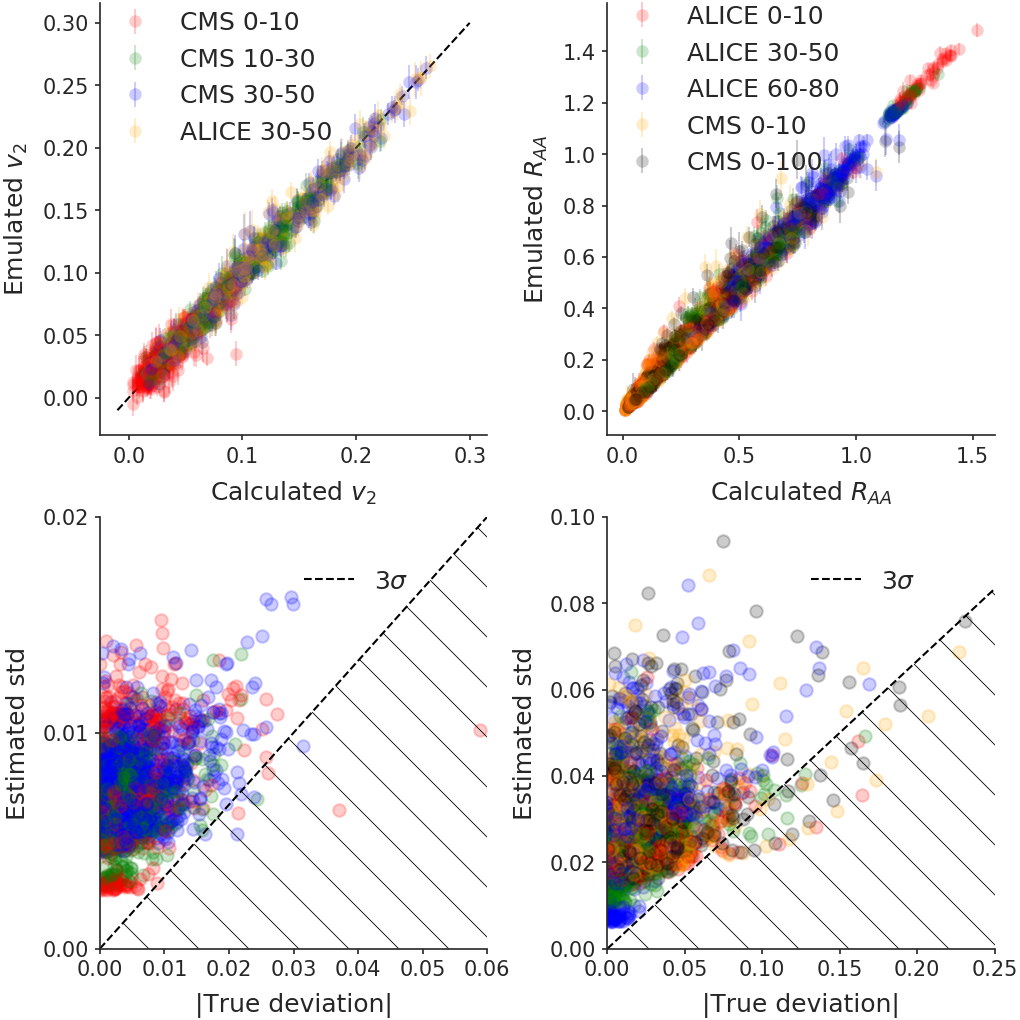
\includegraphics[width=\textwidth]{New-analysis/validation.png}
\caption{•}
\label{fig:new:validation}
\end{figure}

\paragraph{Co-variance matrix} Now we specify the covariance matrix to define the likelihood function, and marginalize the posterior distribution function using the MCMC technique.
The general structure of the covariance matrix has been introduced in the previous section, here we use a centrality decorrelation factor $C=0.5$, and choses two different $\ln p_T$ correlation length $0.5$ and $1$ to how sensitive the calibration is to different form of covariance matrix.
We first take a look at the global level of agreement between the calibrated model and the data.
In figure 

\begin{figure}
\centering
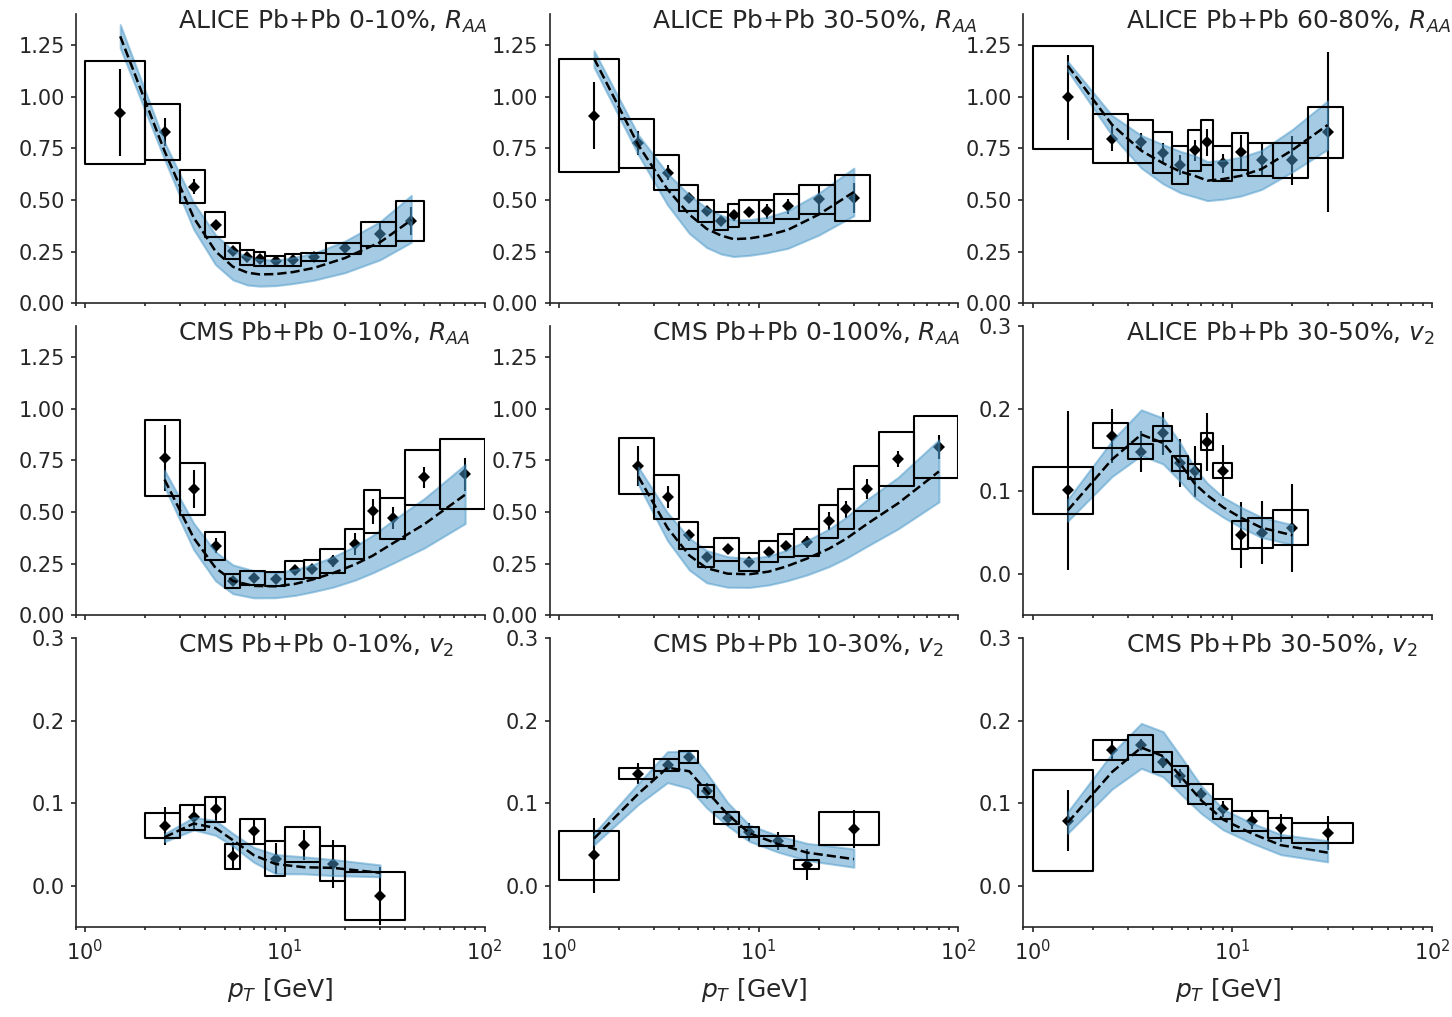
\includegraphics[width=\textwidth]{New-analysis/obs_posterior.png}
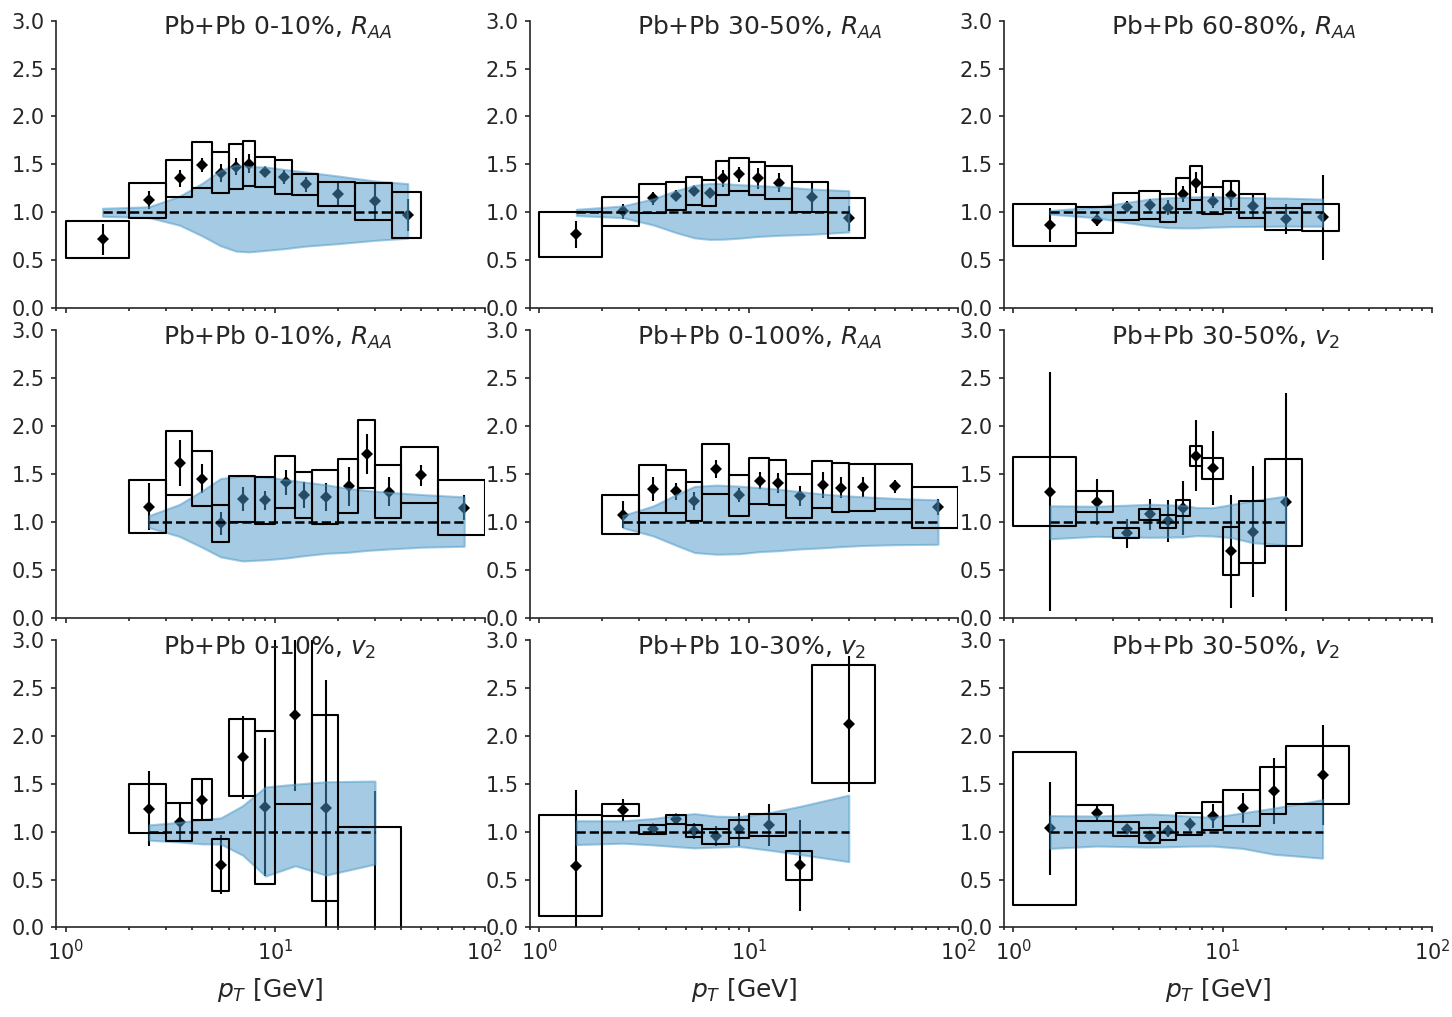
\includegraphics[width=.98\textwidth]{New-analysis/obs_ratio_posterior.png}
\caption{•}
\label{fig:new:obs_posterior}
\end{figure}

\begin{figure}
\centering
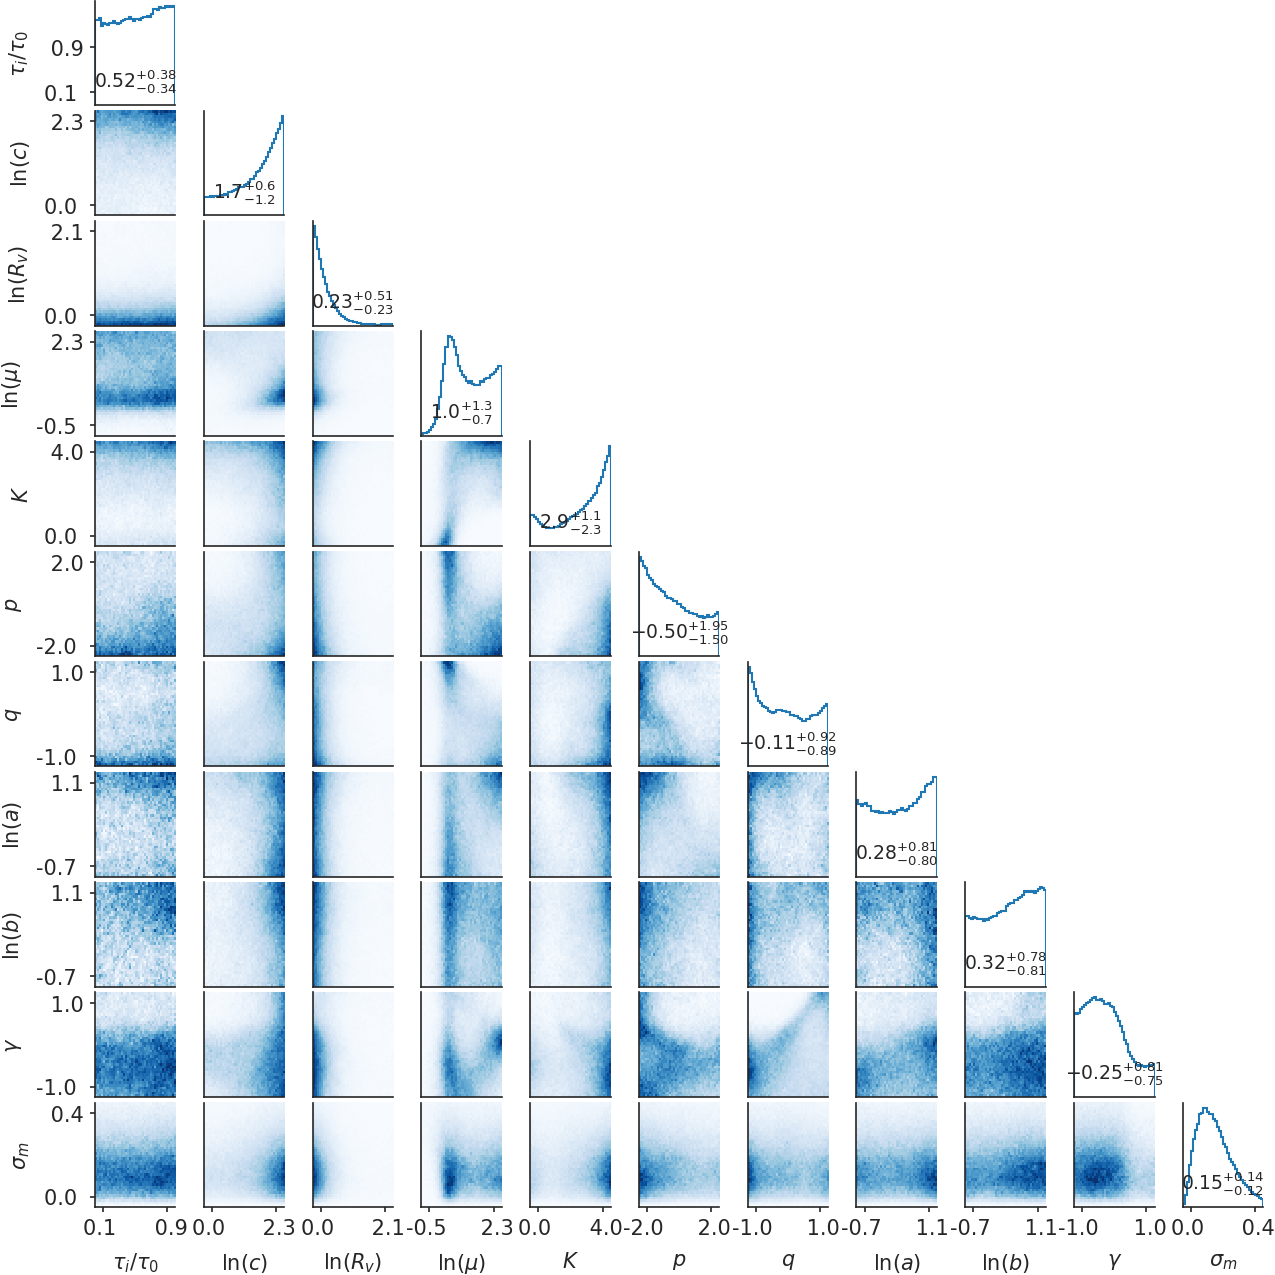
\includegraphics[width=\textwidth]{New-analysis/posterior-L0d3.png}
\caption{•}
\label{fig:new:posterior-l0d3}
\end{figure}

\begin{figure}
\centering
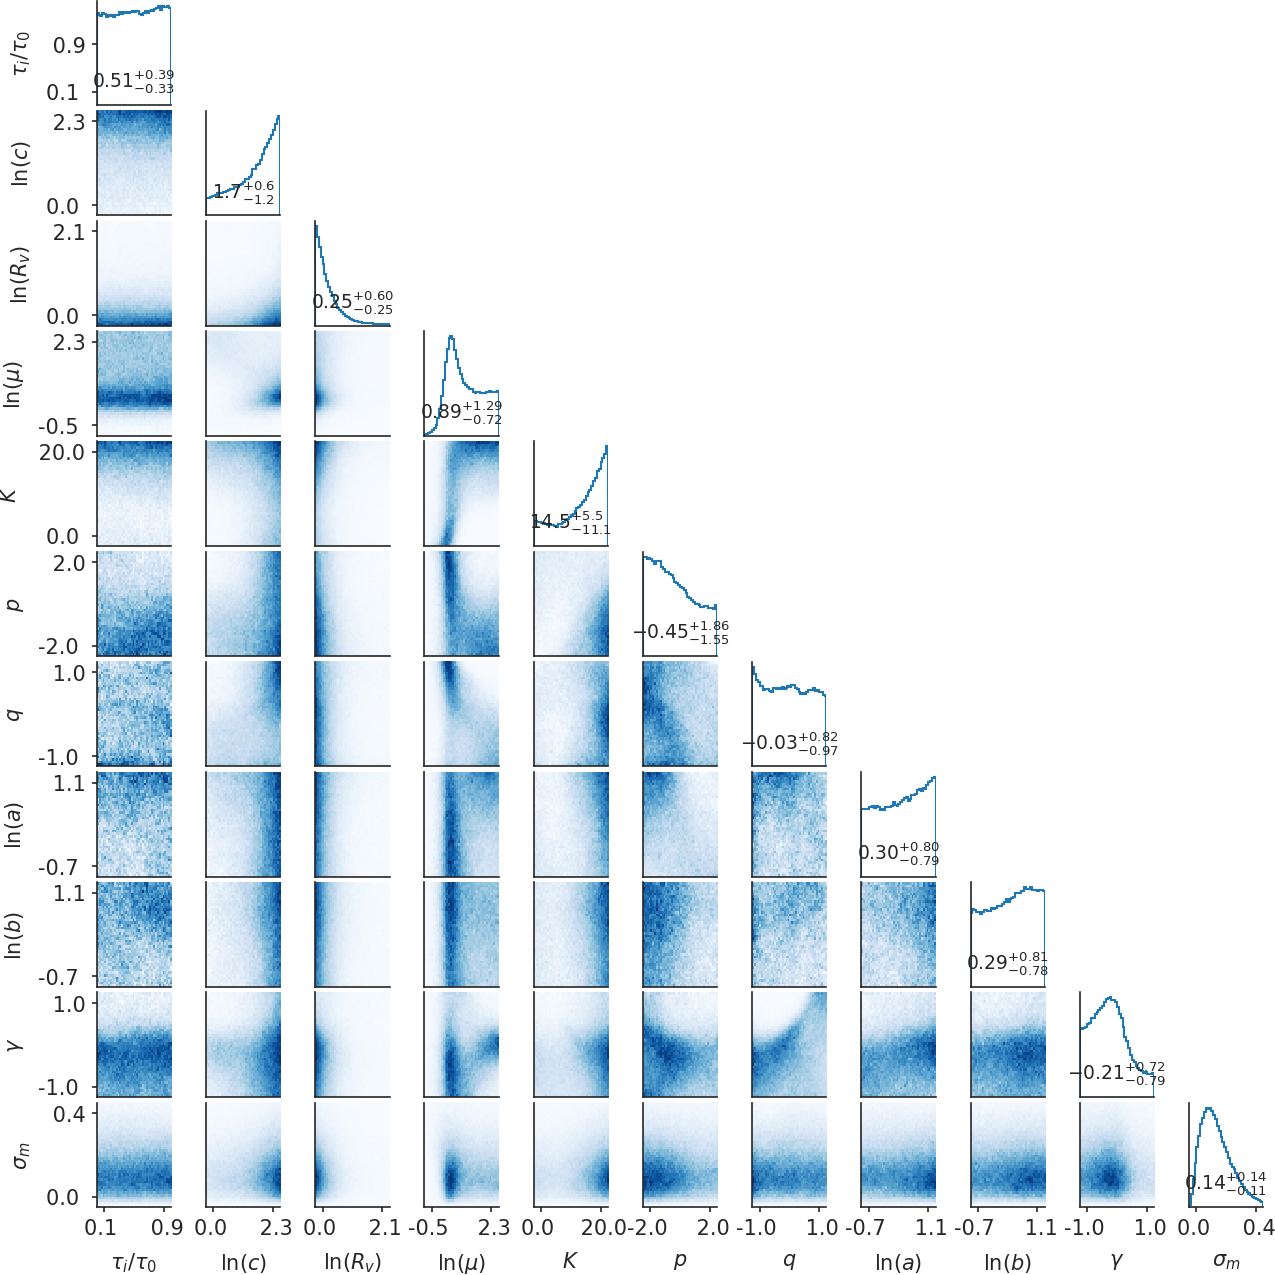
\includegraphics[width=\textwidth]{New-analysis/posterior-L0d5.png}
\caption{•}
\label{fig:new:posterior-l0d5}
\end{figure}

\begin{figure}
\centering
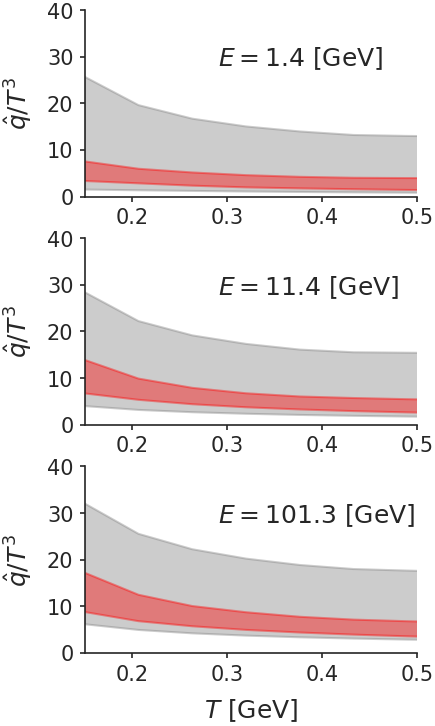
\includegraphics[width=.5\textwidth]{New-analysis/qhat_posterior.png}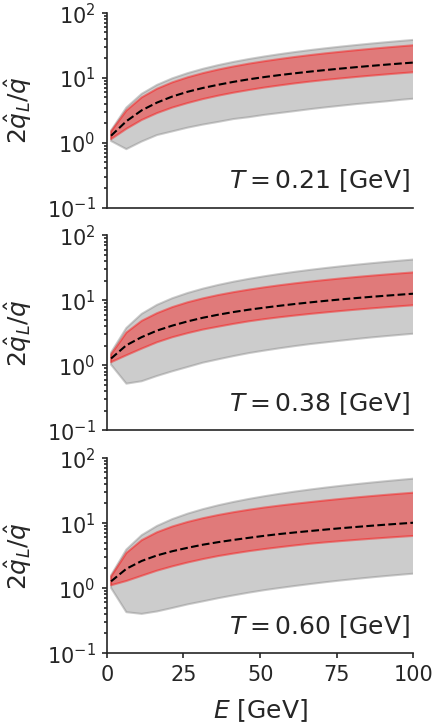
\includegraphics[width=.5\textwidth]{New-analysis/ER_posterior.png}
\caption{•}
\label{fig:new:posterior-qhat}
\end{figure}

\begin{figure}
\centering
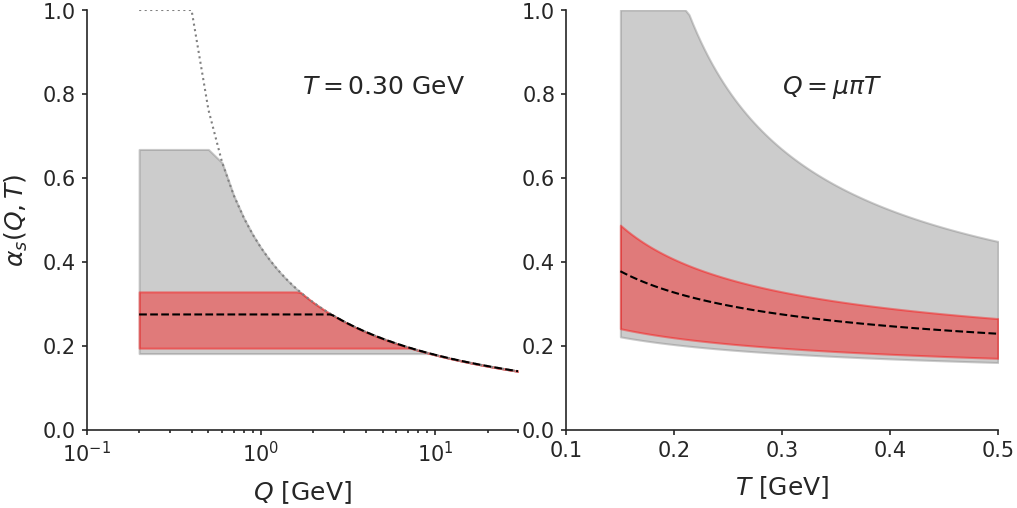
\includegraphics[width=.6\textwidth]{New-analysis/alpha_s_posterior.png}
\caption{•}
\label{fig:new:posterior-alphas}
\end{figure}
